\subsection{Test of image identification} \label{sec:tests.t1}

The first post-modelling test was a qualitative comparison of the
original arrival-time surfaces and the input spaghetti diagrams given
by the modeller.  This tested first, for correct identification and
location of the lensed images, and second, the correct parities and
ordering for the lensed images in respect of the arrival time.

While we expected the identification of lensed images to be trivial,
given the generally clean appearance of the sims in the test, we
expected the parities and time-ordering to be more difficult.  While
the \spl tutorials had provided some general rules of thumb, to be
consistently correct with the time-ordering, a modeller needs to
develop some intuition for arrival time surfaces.  This is an area
where experience and tutorials training could improve results at a
later stage, and correspondingly, feedback on the difficulties
modellers encounter can help improve the tutorial materials.

\tabref{stats} presents a summary of the test.  The evaluation was
done manually, comparing the input to \spl with the actual
arrival-time surface of the sim.  This amounts to comparing the
upper-left and middle-left panels in each of
Figures~\ref{fig:6941}--\ref{fig:7022}, and similaly the other 113
models.

\begin{table}\centering\begin{tabular}{llcc}\hline
     & Total & 119 \\
\hline
 R1: & images approximately on correct locations & 110 \\
 R2: & images parities and time-ordering correct & 70 \\
\hline
 E01: & inaccurate image placement over an arc & 21 \\
 E02: & swapped minimum and saddle in double  & 2 \\
 E03: & identified two images of four & 5 \\
 E04: & modelled a three-image arc as one image & 4 \\
 E05: & swapped early and late saddles in a quad & 7 \\
 E06: & swapped minima and saddles in quad & 38 \\
 E07: & missed faint images & 1 \\
 E08: & modelled one image as a three-image arc & 5 \\
 E09: & identified two nearby images as one & 3 \\
 E10: & proposed too many images & 1 \\
\hline
\end{tabular}
\caption{Table of image-identification errors and the number of models
  containing each.}
\label{tab:stats}
\end{table}

The images of the system are considered to be identified correctly, if all the images have been identified and are approximated within $\pm0.05\cdot\text{imgage width}$.
The parity is considered correct, if those identified points have the right ordering with respect to arrival time.

Additionally, ten types of errors (labeled E01 -- E10, listed in \tabref{stats}) that occurred were identified.
Each generated model could contain more than one error.



We conclude that the volunteers are performing very well identifying and positioning images, with a performance of 92\% (R1, p=0.92).
Most of the problems where due to unclear arc-like structures (E01, p=0.18; E04, p=0.03; E08, p=0.04).
Critical errors like the failure to identify all five images in a five images system (E03, p=0.04) or to include too many images (E10, p=0.01) did almost never happen.
From this we conclude that the introduction materials was adequate and the volunteers understand the basics of gravitational lensing.

The assignment of the parity of the images was a more difficult task.
In 59\% (R2, p=0.59, N=70) of the cases the volunteers succeeded to identify the right configuration.
Most of the failures are due to E06 (N=38, p=32\%), followed by E05 (N=7, p=6\%).
E06 describes a situation, where the minima and saddle points of a five image configuration were exchanged (rotated by $\pm90\dgr$), see \figref{7022} for an example.
E05 describes a situation, where the ordering of the saddle points was wrong (rotation by $180\dgr$).
While these errors occurred, we suspect they can be avoided with better training material and some examples for the obvious cases.
For more challenging cases, like very symmetrical distribution of the lensed images (for example model 7022, \figref{7022}), those errors should still produce plausible results, as will be explained in the next section.

\FloatBarrier

\subsection{Test of mass-profile recovery} \label{sec:tests.t2}

The second test was to compare the mass distributions of the lens $\kappa(x, y)$ given by the sims and generated by the volunteers.
To get a means of comparing the sims to the models, the total convergence\footnote{often called enclosed mass} $\kappa_{\text{encl}}(r)$ was calculated for both.
The Einstein radius $\Theta_\text{E}$ is defined by $\kappa_{\text{encl}}(\Theta_\text{E})=1$ and gives a number that allows a rough comparison between a sim and a model.
We also let an expert (PS) model three selected systems to compare the results from volunteers to those of a professional.


To compare the enclosed mass profile and the Einstein radius of the simulation and the models, \kenc was calculated using the mass map \kap[x,y] generated in the modeling process.
From the ensemble of models generated by one modeling process, the mean is taken as the resulting $\kappa(r)$ to calculate \ERg.
To estimate the errors, the extremal models are used to estimate a lower and upper limit for \ERg.
These results can be seen in \figref{ER_per_sim}.
This figure shows that this technique of estimating the error using the ensemble of all models underestimates the error significantly and should be improved for further analysis.

\begin{figure*}
  \centering
    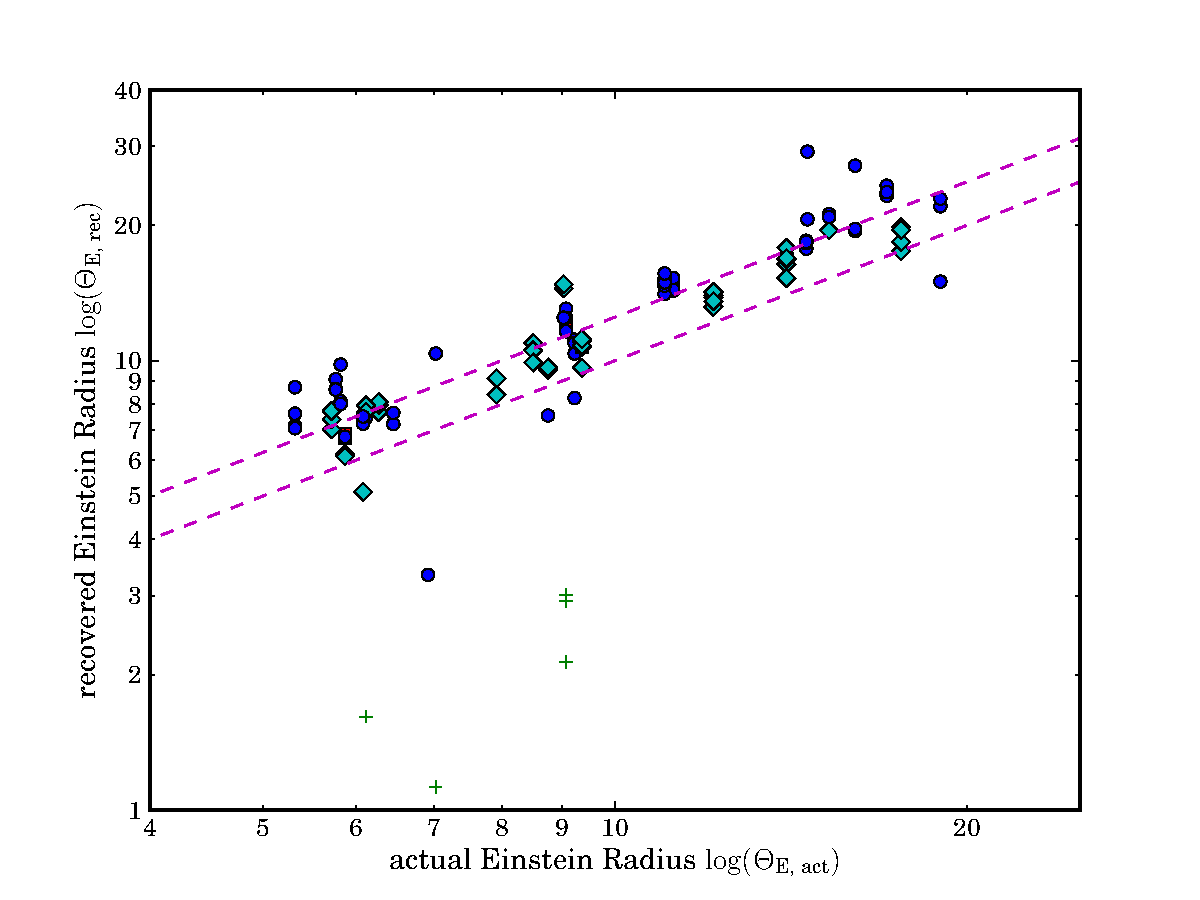
\includegraphics[width=0.90\linewidth]{fig/eR_5}
  \caption{Relative \ERf / \ERg[, sim] for models by volunteers (blue cross), models made by an expert (red cross with offset), including rejected models (green squares); binned per sim.}
  \label{fig:ER_per_sim}
\end{figure*}



\Figref{ER_per_sim} shows that the calculated \ERf of the models tend
to be too high.  The overshoot varies from around 0.2 to 0.4 for good
models.  Discounting the models which were flagged by the users as
poor, \ERf{E,rec} is overestimated.  The mean and standard deviation
of the overestimate are 25\% and 20\%.  The models by an expert also
show a similar bias, having mean and standard deviation of the
overestimate being 20\% and 8\%.
One of the reasons for this is that it is hard to get the center of the lens on spot.
An offset leads to a flatter mass profile for the model compared to the simulation.

Comparing the models from volunteers and experts can be done in Figures \ref{fig:7022}, \ref{fig:7025} and \ref{fig:kapenc_compare_faulty}, where only the
expert got the right configuration (\figref{7022}) but enclosed masses are all fairly similar.  In cases with nearly symmetric image configurations, like this example, it is more difficult to identify the image parities correctly.  Incorrect image-parity identification changes the orientation of the mass distribution \kap[x,y],
but \kenc and thus the \ERf are not influenced that much.

Two additional sims were modeled by an expert, \asw{1hpf} and \asw{0vqg}.
Looking at the results for \ERg for those models in \figref{ER_per_sim}, we conclude that the performance of volunteers (blue crosses) and experts (red crosses, offset) is comparable.
%Note that the models of \asw{0vqg} with \ERg[, rel] around 0.25 (6935 -- 6937) are failed models that show the attempts of a single user, that came finally up with model 6938 as final result.\todo{remove?}

\section{Outlook} \label{sec:todo}

The lens-modeling challenge indicates that the Spacewarps collective
is good, not only for identifying lens candidates for follow-up, but
modeling candidates as well.

There is, however, plenty of room for improvement.

First, the particular modeling strategy implemented is not the only
one possible.  \spl requires modelers to characterize the overall
image structure in abstract terms based on Fermat's principle, and the
placement of mass distributions is done by the computer.  In other
modeling tools, the user puts down a trial mass distribution and has
the machine refine it.  A few of these modeling programs have also
been designed with citizen science in mind, and would be interesting
in the Spacewarps environment.

Second, \spl needs some enhancements.

\begin{itemize}
\item Currently, \spl does not attempt to model the source shape; the
  user identifies the brightest points on the image, and these are
  taken as images of a point-like source, whose positions must be
  reproduced exactly. For generating a synthetic image, a conical
  source profile is assumed. Fitting for the source profile to
  optimize resemblance to the observed lensed image after the lens
  model has been generated, is algorithmically straightforward
  \citep[cf.][]{2003ApJ...590..673W,2006MNRAS.371..983S} and planned
  to be implemented.  This would alleviate another problem with \spl,
  which is that there is no numerical figure of merit, and assessment
  of a model is a judgment call based on the synthetic image, and on
  whether the mass distribution and the arrival-time surface show
  suspect features.
\item \spl has a tendency to somewhat overestimate the Einstein radius
  (evident from Figure \ref{fig:ER_per_sim}), and it is also apparent
  that the models tend to be too shallow.  This possible explanation
  is that, while the sims are steeply peaked at the centre, the
  pixellated mass model fixes a comparatively large area near the
  central at constant density.  One way to solve this problem would be
  to introduce smaller pixels in the central region, thus enabled a
  steeper centre.
\item Another limitation so far in \spl is that the lens is assumed to
  be dominated by one galaxy, which puts most galaxy-group lenses
  beyond the reach of the modeler. Since complicated group lenses are
  some of the most interesting candidates present, removing this
  limitation is most desirable.  From the users' point of view, it
  would mean that spaghetti contours with more than one maximum can be
  allowed.  For examples, see Figure 5c in \citep{2001ApJ...557..594R}
  and Figure 4b in \cite{2003ApJ...590...39K}.
\item At present, a single false-color composite is used as the data.
  An option could be added to use all available filters, individually
  or in combination, at the user wishes.
\end{itemize}

The third desirable avenue of improvement is to facilitate
collaborative work.

\begin{itemize}
\item As mentioned above, the option of revising an already-archived
  model is already available.  Desired now are tools for comparing
  different models of a given system, both visually and through
  different statistical measures.  As evidenced by a current
  collaborative modeling effort, a particularly interesting candidate
  can lead to an extended discussion and dozens of models.
\item Better tutorial materials are also needed, and this would
  address some of the problem areas found in the modeling challenge.
  For example, we saw in \secref{tests.t1} that volunteers are most
  prone to making errors in two situations: when in identifying an arc-
  like structure while placing the points, and in identifying the
  correct ordering of the points in nearly-symmetric configurations.
\end{itemize}

The \spl program was developed by Kueng, with design suggestions from
Coles, Cornen and Saha, and feedback from all co-authors.  The
simulations were created by A.~More, in consultation with Marshall,
S.~More and Verma.  Modelling was done by Baeten, Cornen, McMillan,
Odermatt, Saha and Wilcox, with post-modelling analysis by Kueng and
Saha.  All authors participated in writing and editing the manuscript.

\section{Acknowledgments}

We thank the Swiss Society for Astrophysics and Astronomy and the
Swiss Academy of Sciences. AV is supported by a research fellowship
from the Leverhulme Trust.

\clearpage

